%!TEX root=../../autopilot.tex
\section{Hardware}
\label{sec:hardware}

The Raspberry Pi can interface with nearly all common hardware, and has an \href{https://www.raspberrypi.org/help/}{extensive collection} of \href{https://elinux.org/RPi_Guides}{guides}, \href{https://elinux.org/RPi_Tutorials}{tutorials}, and an active \href{https://www.raspberrypi.org/forums/}{forum} to support users implementing new hardware. There is also an enormous amount of existing hardware for the Raspberry Pi, including \href{https://www.hifiberry.com/}{sound cards}, \href{https://www.adafruit.com/product/2348}{motor controllers}, \href{https://www.digikey.com/product-detail/en/raspberry-pi/SENSE-HAT/1690-1013-ND/6196429}{sensor arrays}, \href{https://www.seeedstudio.com/Raspberry-Pi-High-Precision-AD-DA-Board-p-2765.html}{ADC/DACs}, and \href{https://www.digikey.com/product-detail/en/pimoroni-ltd/PIM369/1778-1221-ND/9521981}{touchscreen displays}, largely eliminating the need for a separate ecosystem of purpose-built hardware (Table \ref{tab:periphs}). 

\begin{margintable}[-0.75cm]
\caption{
\textbf{Cost of common peripherals.} The native hardware of the Raspberry Pi, low-level hardware control of Autopilot, and availability of inexpensive off-the-shelf components compatible with the raspi make most custom-built peripherals unnecessary.}
\label{tab:periphs}
\noindent\begin{tabularx}{\linewidth}{Rll}
\toprule
\textbf{Device} & Raspi & Bpod \\
\midrule
HiFiBerry DAC2 Pro & \href{https://www.hifiberry.com/shop/boards/hifiberry-dac2-pro/}{\$45} &  \href{https://sanworks.io/shop/viewproduct?productID=1032}{\$445}\\
ADC & \href{https://thepihut.com/products/high-precision-adc-hat-for-raspberry-pi-10-channel-32-bit}{\$30} & \href{https://sanworks.io/shop/viewproduct?productID=1021}{\$495}\\
I2C & \$0 & \href{https://sanworks.io/shop/viewproduct?productID=1019}{\$225} \\
Ethernet & \$0 & \href{https://sanworks.io/shop/viewproduct?productID=1025}{\$285} \\
Rotary Encoder & \$0 &  \href{https://sanworks.io/shop/viewproduct?productID=1022}{\$145}\\
\bottomrule
\end{tabularx}
\end{margintable}

\begin{marginfigure}[0cm]
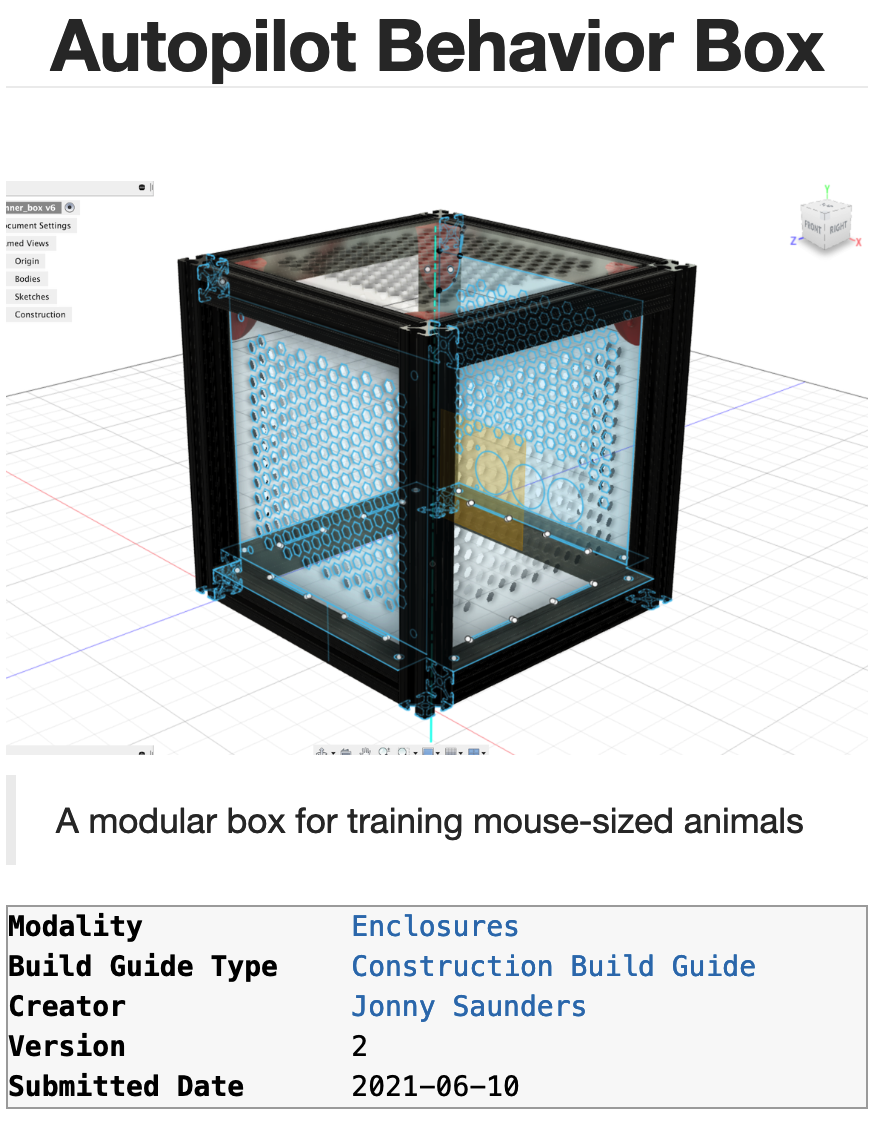
\includegraphics[width=\linewidth]{autopilot/autopilot/src/figures/behavior_box.png}
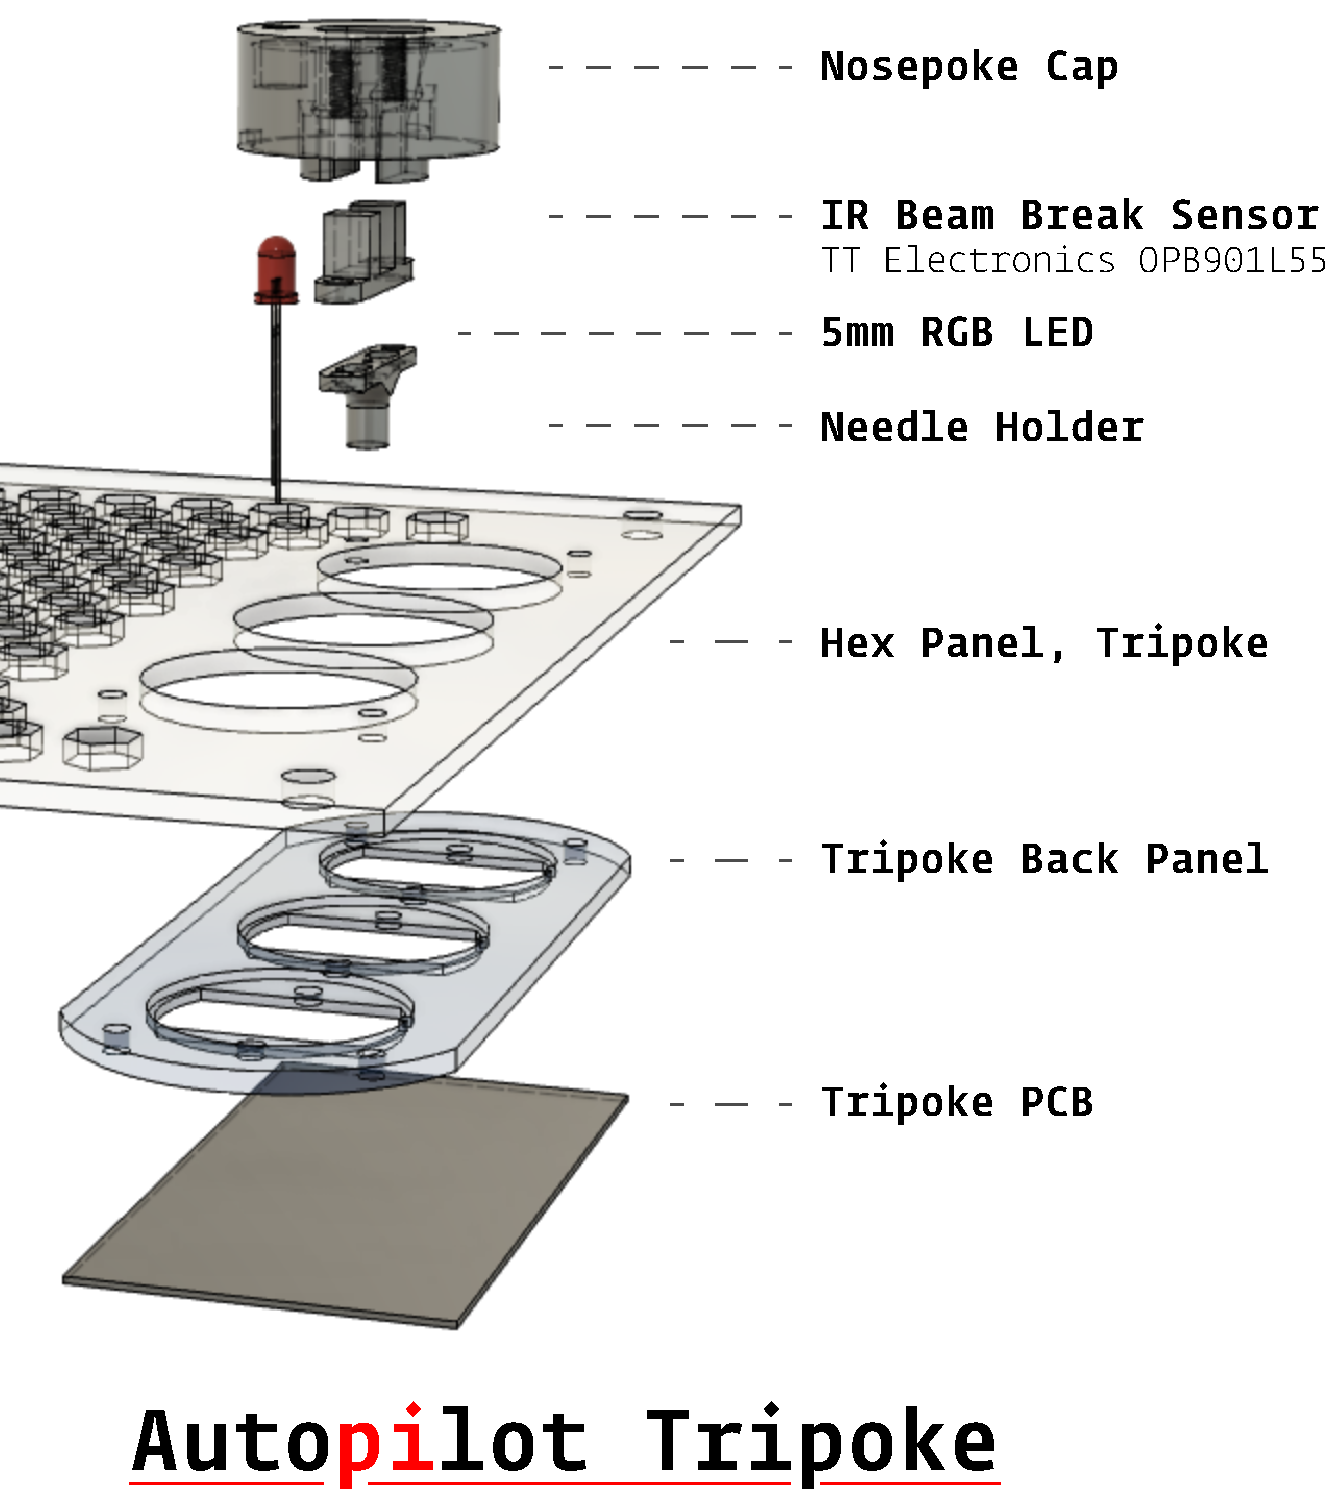
\includegraphics[width=\linewidth]{autopilot/autopilot/src/figures/tripoke_assembly_order.pdf}
\caption{Two examples of parts with assembly guides available on the autopilot wiki: A modular \href{https://wiki.auto-pi-lot.com/index.php/Autopilot_Behavior_Box}{behavior box} with magnetic snap-in panels (top), and a \href{https://wiki.auto-pi-lot.com/index.php/Autopilot_Tripoke}{three-nosepoke panel} (bottom).}
\label{fig:pokeport}
\end{marginfigure}%

Autopilot controls hardware with an extensible inheritance hierarchy of Python classes intended to be built into a library of hardware controllers analogously to tasks. Autopilot uses \href{http://abyz.me.uk/rpi/pigpio/}{pigpio} to interact with its GPIO pins, giving Autopilot $5 \mu s$ measurement precision and enabling protocols that require high precision (such as Serial, PWM, and I2C) for nearly all of the pins.  Currently, Autopilot also has a family of objects to control cameras (both the \href{https://docs.auto-pi-lot.com/en/latest/hardware/cameras.html\#autopilot.hardware.cameras.PiCamera}{Raspberry Pi Camera} and \href{https://docs.auto-pi-lot.com/en/latest/hardware/cameras.html\#autopilot.hardware.cameras.Camera_Spinnaker}{high-speed GENICAM-compliant} cameras), i2c-based \href{https://docs.auto-pi-lot.com/en/latest/hardware/i2c.html\#autopilot.hardware.i2c.I2C_9DOF}{motion} and \href{https://docs.auto-pi-lot.com/en/latest/hardware/i2c.html\#autopilot.hardware.i2c.MLX90640}{heat} sensors, and \href{https://docs.auto-pi-lot.com/en/latest/hardware/usb.html\#autopilot.hardware.usb.Wheel}{USB mice}.  In the \hyperref[sec:future]{future} we intend to improve performance further by replacing time-critical hardware operations with low-level interfaces written in Rust.

\begin{table}[ht!]
\caption{Specifications of reviewed behavior hardware. BPod's state machine uses the Teensy 3.6 microcontroller, and PyControl uses the Micropython Pyboard.}
\label{hwtab}
\begin{tabularx}{\linewidth}{Rp{3.5cm}p{2cm}p{2cm}}\toprule
& \href{https://www.raspberrypi.org/products/raspberry-pi-4-model-b/specifications/}{\textbf{Raspberry Pi 4B}} & \href{https://www.pjrc.com/teensy/techspecs.html}{\textbf{Teensy 3.6}} & \href{https://micropython.org/}{\textbf{pyboard}}\\
\midrule
CPU Clock & 1.5GHz & 180MHz & 168MHz \\
CPU Cores & 4 & 1 & 1 \\
Architecture & ARMv8-A, 64-bit & ARMv7 32-bit & ARMv7 32-bit \\
RAM Size & 2, 4, or 8GB & 256KB & 192KB\\
Storage & MicroSD (any size) & 1024KB & 1024KB \\
GPU & Broadcom VideoCore VI & \textcolor{red}{---} & \textcolor{red}{---} \\
GPIO Pins & 40 & 58 & 29 \\
USB Ports & 2x USB 2.0, 2x USB 3.0  & 2x USB 2.0 & 1x USB 2.0 \\
Ethernet & 1Gbps & 100Mbps & \textcolor{red}{---} \\
WiFi & 2.4/5 GHz b/g/n/ac & \textcolor{red}{---} & \textcolor{red}{---} \\
Camera & 15-pin Serial Interface & \textcolor{red}{---} & \textcolor{red}{---} \\
Bluetooth & \checkmark & \textcolor{red}{---} & \textcolor{red}{---} \\
\end{tabularx}
\end{table}

To organize and make available the vast amount of contextual knowledge needed to build and use experimental hardware, we have made a densely linked and publicly editable \href{https://wiki.auto-pi-lot.com/index.php/Autopilot_Wiki}{semantic wiki}. The Autopilot wiki contains, among others, reference information for \href{https://wiki.auto-pi-lot.com/index.php/Parts}{off-the-shelf parts}, schematics for \href{https://wiki.auto-pi-lot.com/index.php/2D_CAD}{2D} and \href{https://wiki.auto-pi-lot.com/index.php/3D_CAD}{3D}-printable components, and \href{https://wiki.auto-pi-lot.com/index.php/Guides}{guides} for building experimental apparatuses and custom parts. The wiki combines unrestrictive freeform editing with structured, computer-readable \href{https://www.semantic-mediawiki.org/wiki/Semantic_MediaWiki}{semantic properties}, and we have defined a collection of \href{https://wiki.auto-pi-lot.com/index.php/Special:CategoryTree?target=Hardware&mode=categories&namespaces=&title=Special%3ACategoryTree}{schemas} for commonly documented items coupled with \href{https://wiki.auto-pi-lot.com/index.php/Special:Forms}{submission forms} for ease of use. For example, the wiki page for the \href{https://wiki.auto-pi-lot.com/index.php/Lee_LHDA0531115H}{Lee Company solenoid} we use has fields from a generic \href{https://wiki.auto-pi-lot.com/index.php/Category:Part}{Part} schema like a datasheet, price, and voltage, but also that it's a 3-way, normally-closed \href{https://wiki.auto-pi-lot.com/index.php/Category:Solenoid}{solenoid}. 

The wiki's blend of structure and freedom breaks apart typically monolithic hardware documentation into a collaborative, multimodal technical knowledge graph. Autopilot can access the wiki through its \href{https://docs.auto-pi-lot.com/en/latest/guide/plugins.html\#the-wiki-api}{API}, and we intend to tighten their integration over time, including automatic configurations for common parts, usage and longevity benchmarks, detecting mutually incompatible parts, and automatically resolving any additional plugins or dependencies needed to use a part.